% Risultati per test a grafo crescente in numero di nodi
    % tutte le versioni sia su diretti che indiretti
        % grafici confronto
        % commenti
    
% Risultati per test a grafo con densità crescente
    % grafico
    % osservazioni e possibii spiegazioni
        % con matrice tempo costante perché ...
        % con BCSR tempo crescente con densità perché ...
        % per densità elevate stessi tempi
        % linea viola bcsr senza ottimizzazioni work balance (inutile)
        


\chapter{Risultati}\label{chap:Risultati}

    In questo capitolo verranno discussi i principali risultati riscontrati durante la fase di testing. 

    Per facilitare la lettura dei grafici, si ricorda che:
    \begin{description}
        \item[{\color{blue}serial}] è la versione seriale, la prima implementata;
        \item[{\color{red}parallel}] è la prima versione parallela, i grafi sono rappresentati tramite matrice di adiacenza;
        \item[{\color{violet}parallelbcsrtc}] è la seconda versione parallela, molto simile alla precedente, viene adattata per la rappresentazione BCSR includendo le ottimizzazioni che quest'ultima consente;
        \item[{\color{YellowOrange}parallelbcsrvc}] è l'ultima versione implementata, la versione \textit{work balanced}, e applica alla versione precedente diverse ottimizzazioni per sfruttare al massimo le risorse computazionali.
    \end{description}

    Nella prima parte metteremo a confronto le varie implementazioni su input in cui il numero di nodi è variabile e la densità è costante. 
    Viceversa, nella seconda parte analizzeremo come la variazione di densità influisce sui tempi di esecuzione.

    \section{Risultati per quantità nodi variabile}

        Di seguito sono riportati due grafici che mettono a confronto le diverse implementazioni sia nel caso di grafi diretti (Figura \ref{fig:exec-time-dir}) che in quello di grafi indiretti (Figura \ref{fig:exec-time-undir}). I grafici rappresentano esclusivamente i tempi di esecuzione dell'algoritmo, sono esclusi quindi i tempi di inizializzazione e salvataggio dei risultati.

        I valori di tutti gli assi sono espressi in scala logaritmica. Altrimenti, vista la grande differenza tra i valori, alcune linee risulterebbero appiattite e sovrapposte, rendendo difficile l'analisi dei risultati.

        Sulle ordinate sono riportati i tempi espressi in millisecondi mentre sulle ascisse il numero di nodi.

        Prima di passare alle osservazioni sui grafici, facciamo notare che non tutte le versioni sono state testate su tutte le istanze a disposizione per i seguenti motivi:
        \begin{itemize}
            \item la versione seriale è risultata essere talmente inefficiente (in termini di tempo) da consentirne l'esecuzione solamente con piccole istanze;
            \item la prima versione parallela, usando la matrice di adiacenza come metodo di rappresentazione dei dati, è risultata limitata nell'utilizzo della memoria al punto da renderne impossibile l'esecuzione su istanze con più di 30mila nodi.
        \end{itemize}

        Dunque, osservando i grafici si nota quanto segue:
        \begin{itemize}
            \item la versione seriale risulta essere competitiva solamente quando si hanno qualche decina di nodi. Dopodiché, qualsiasi versione parallela diventa preferibile;
            \item le versioni parallele, invece, tra di loro hanno tempi comparabili per grafi di piccole dimensioni, mentre per istanze di medie/grandi dimensioni si iniziano a notare delle differenze;
            \item in generale l'implementazione migliore sembrerebbe l'ultima proposta (approccio \textit{work balanced});
            \item la versione parallela con BCSR (linea viola), all'aumentare delle dimensioni del grafo, sembrerebbe avvicinarsi ai tempi della versione parallela con matrice di adiacenza (linea rossa). Purtroppo non è possibile valutare con esattezza il loro comportamento, essendo la prima versione parallela fortemente limitata dal consumo di memoria.            
        \end{itemize}
        






        

        Efficienza del parallelismo: In entrambi i grafi, l'algoritmo parallelo standard risulta significativamente più veloce rispetto alla versione seriale, ma inizia a mostrare i suoi limiti con grafi molto grandi.
        Ottimizzazioni BCSR: Le versioni con ottimizzazioni BCSR, pur essendo competitive per grafi più piccoli o medi, non scalano altrettanto bene per grafi più grandi, specialmente per i grafi indiretti. La versione con compressione delle colonne (BCSR VC) offre un miglioramento rispetto a quella con righe compresse (BCSR RTC), ma presenta comunque limiti evidenti su grafi di grandi dimensioni.
        Comportamento diverso tra grafi diretti e indiretti: I grafi indiretti sembrano stressare di più le versioni ottimizzate, con un peggioramento delle prestazioni molto marcato all'aumentare delle dimensioni del grafo.
    
    
    
    
    
    
    \section{Risultati per densità variabile}

    

    \begin{figure}
        \centering
        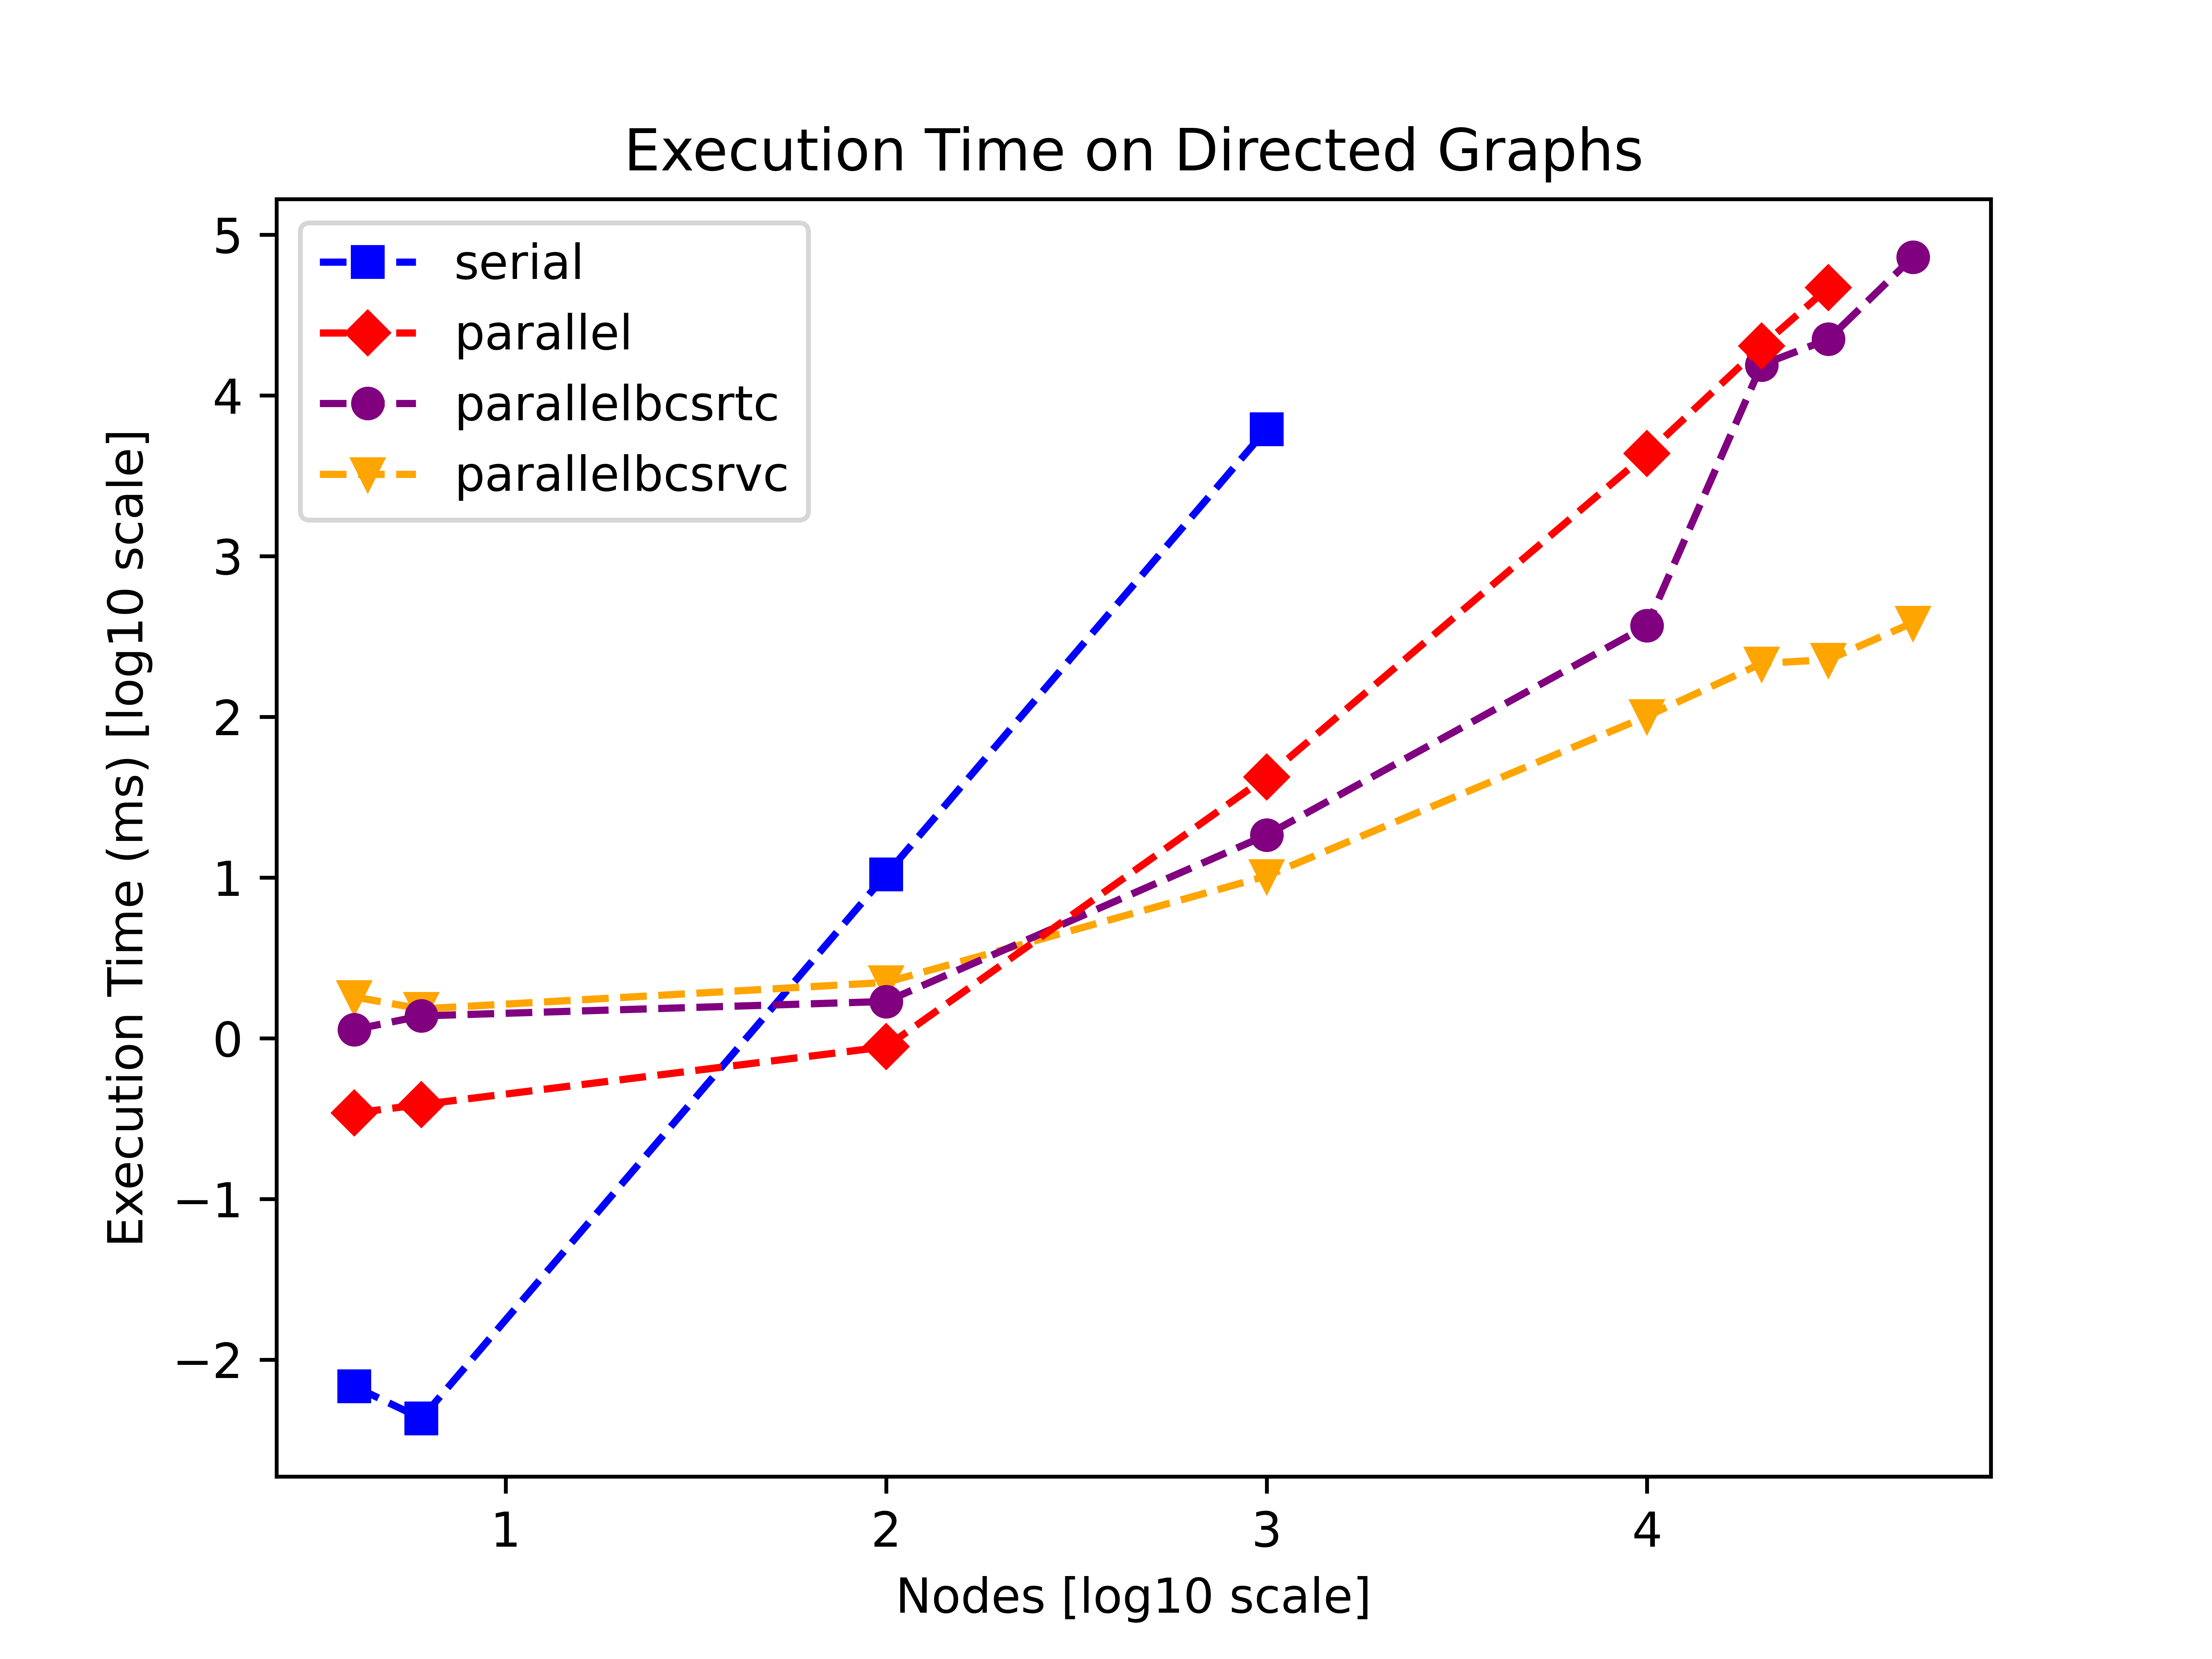
\includegraphics[width=0.7\linewidth]{images/execution_time_directed.png}
        \caption{Tempo di esecuzione dei vari algoritmi con grafi diretti}
        \label{fig:exec-time-dir}
    \end{figure}

    \begin{figure}
        \centering
        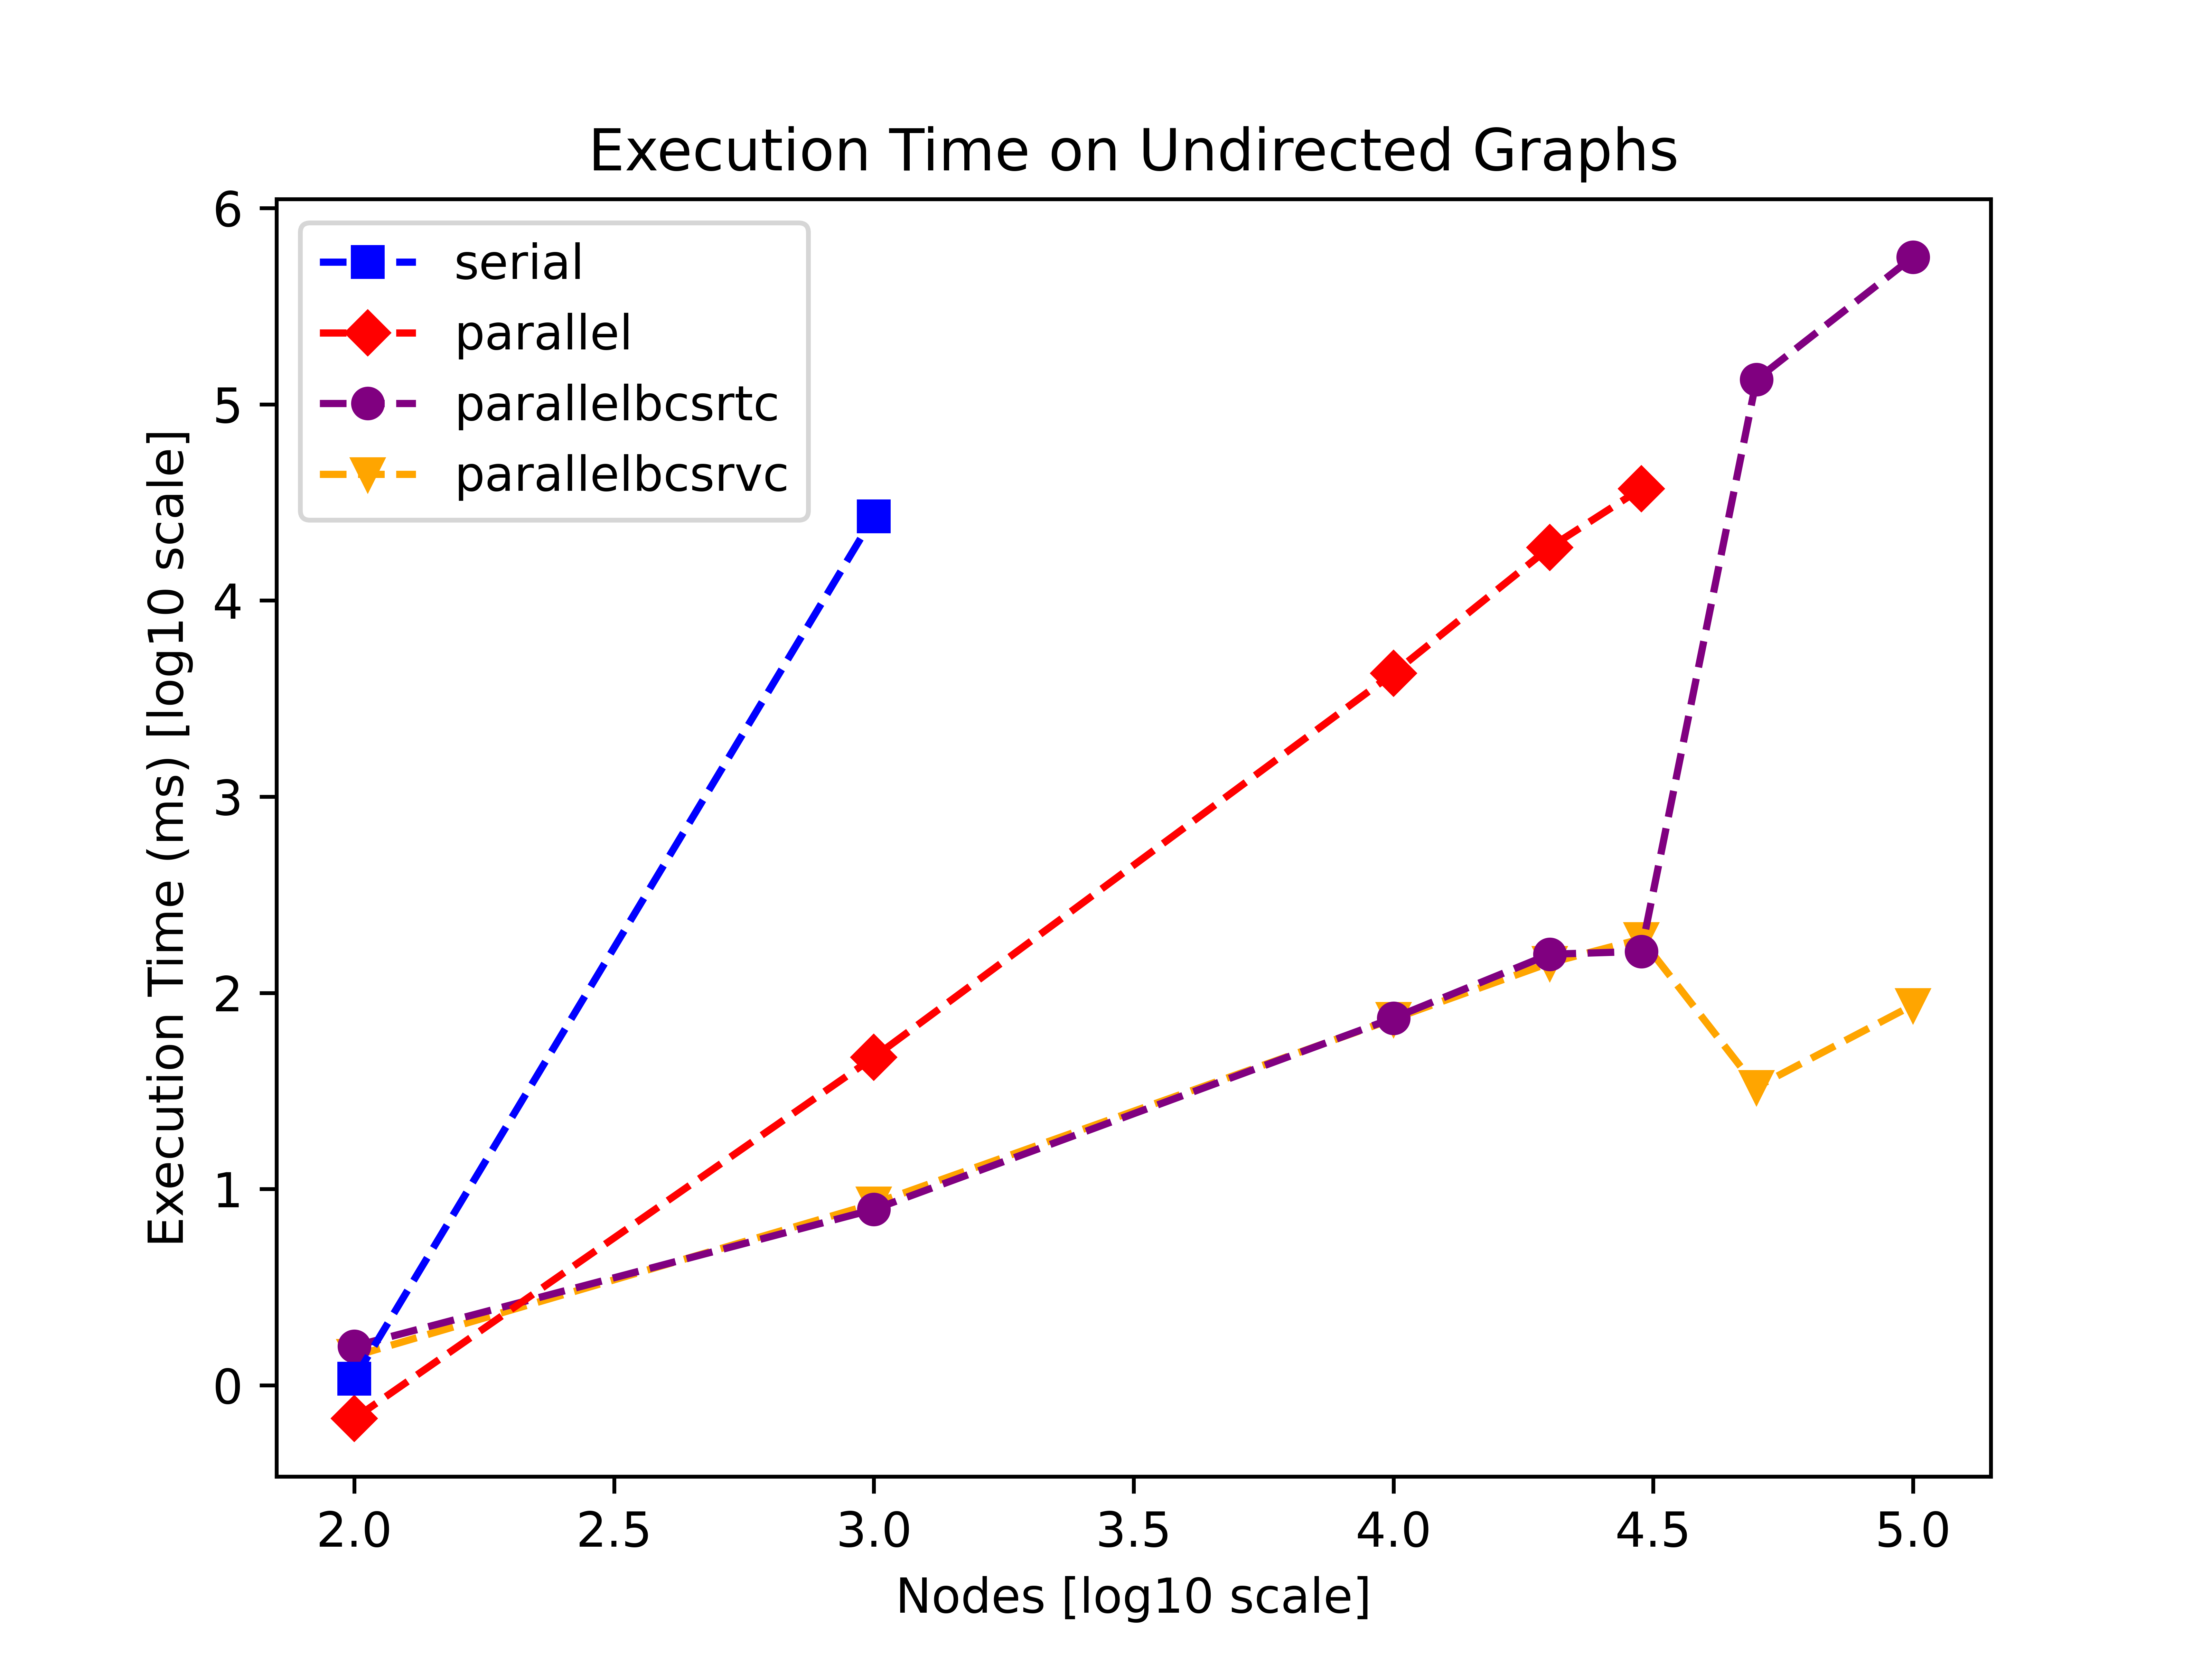
\includegraphics[width=0.7\linewidth]{images/execution_time_undirected.png}
        \caption{Tempo di esecuzione dei vari algoritmi con grafi non diretti}
        \label{fig:exec-time-undir}
    \end{figure}

    \begin{figure}
        \centering
        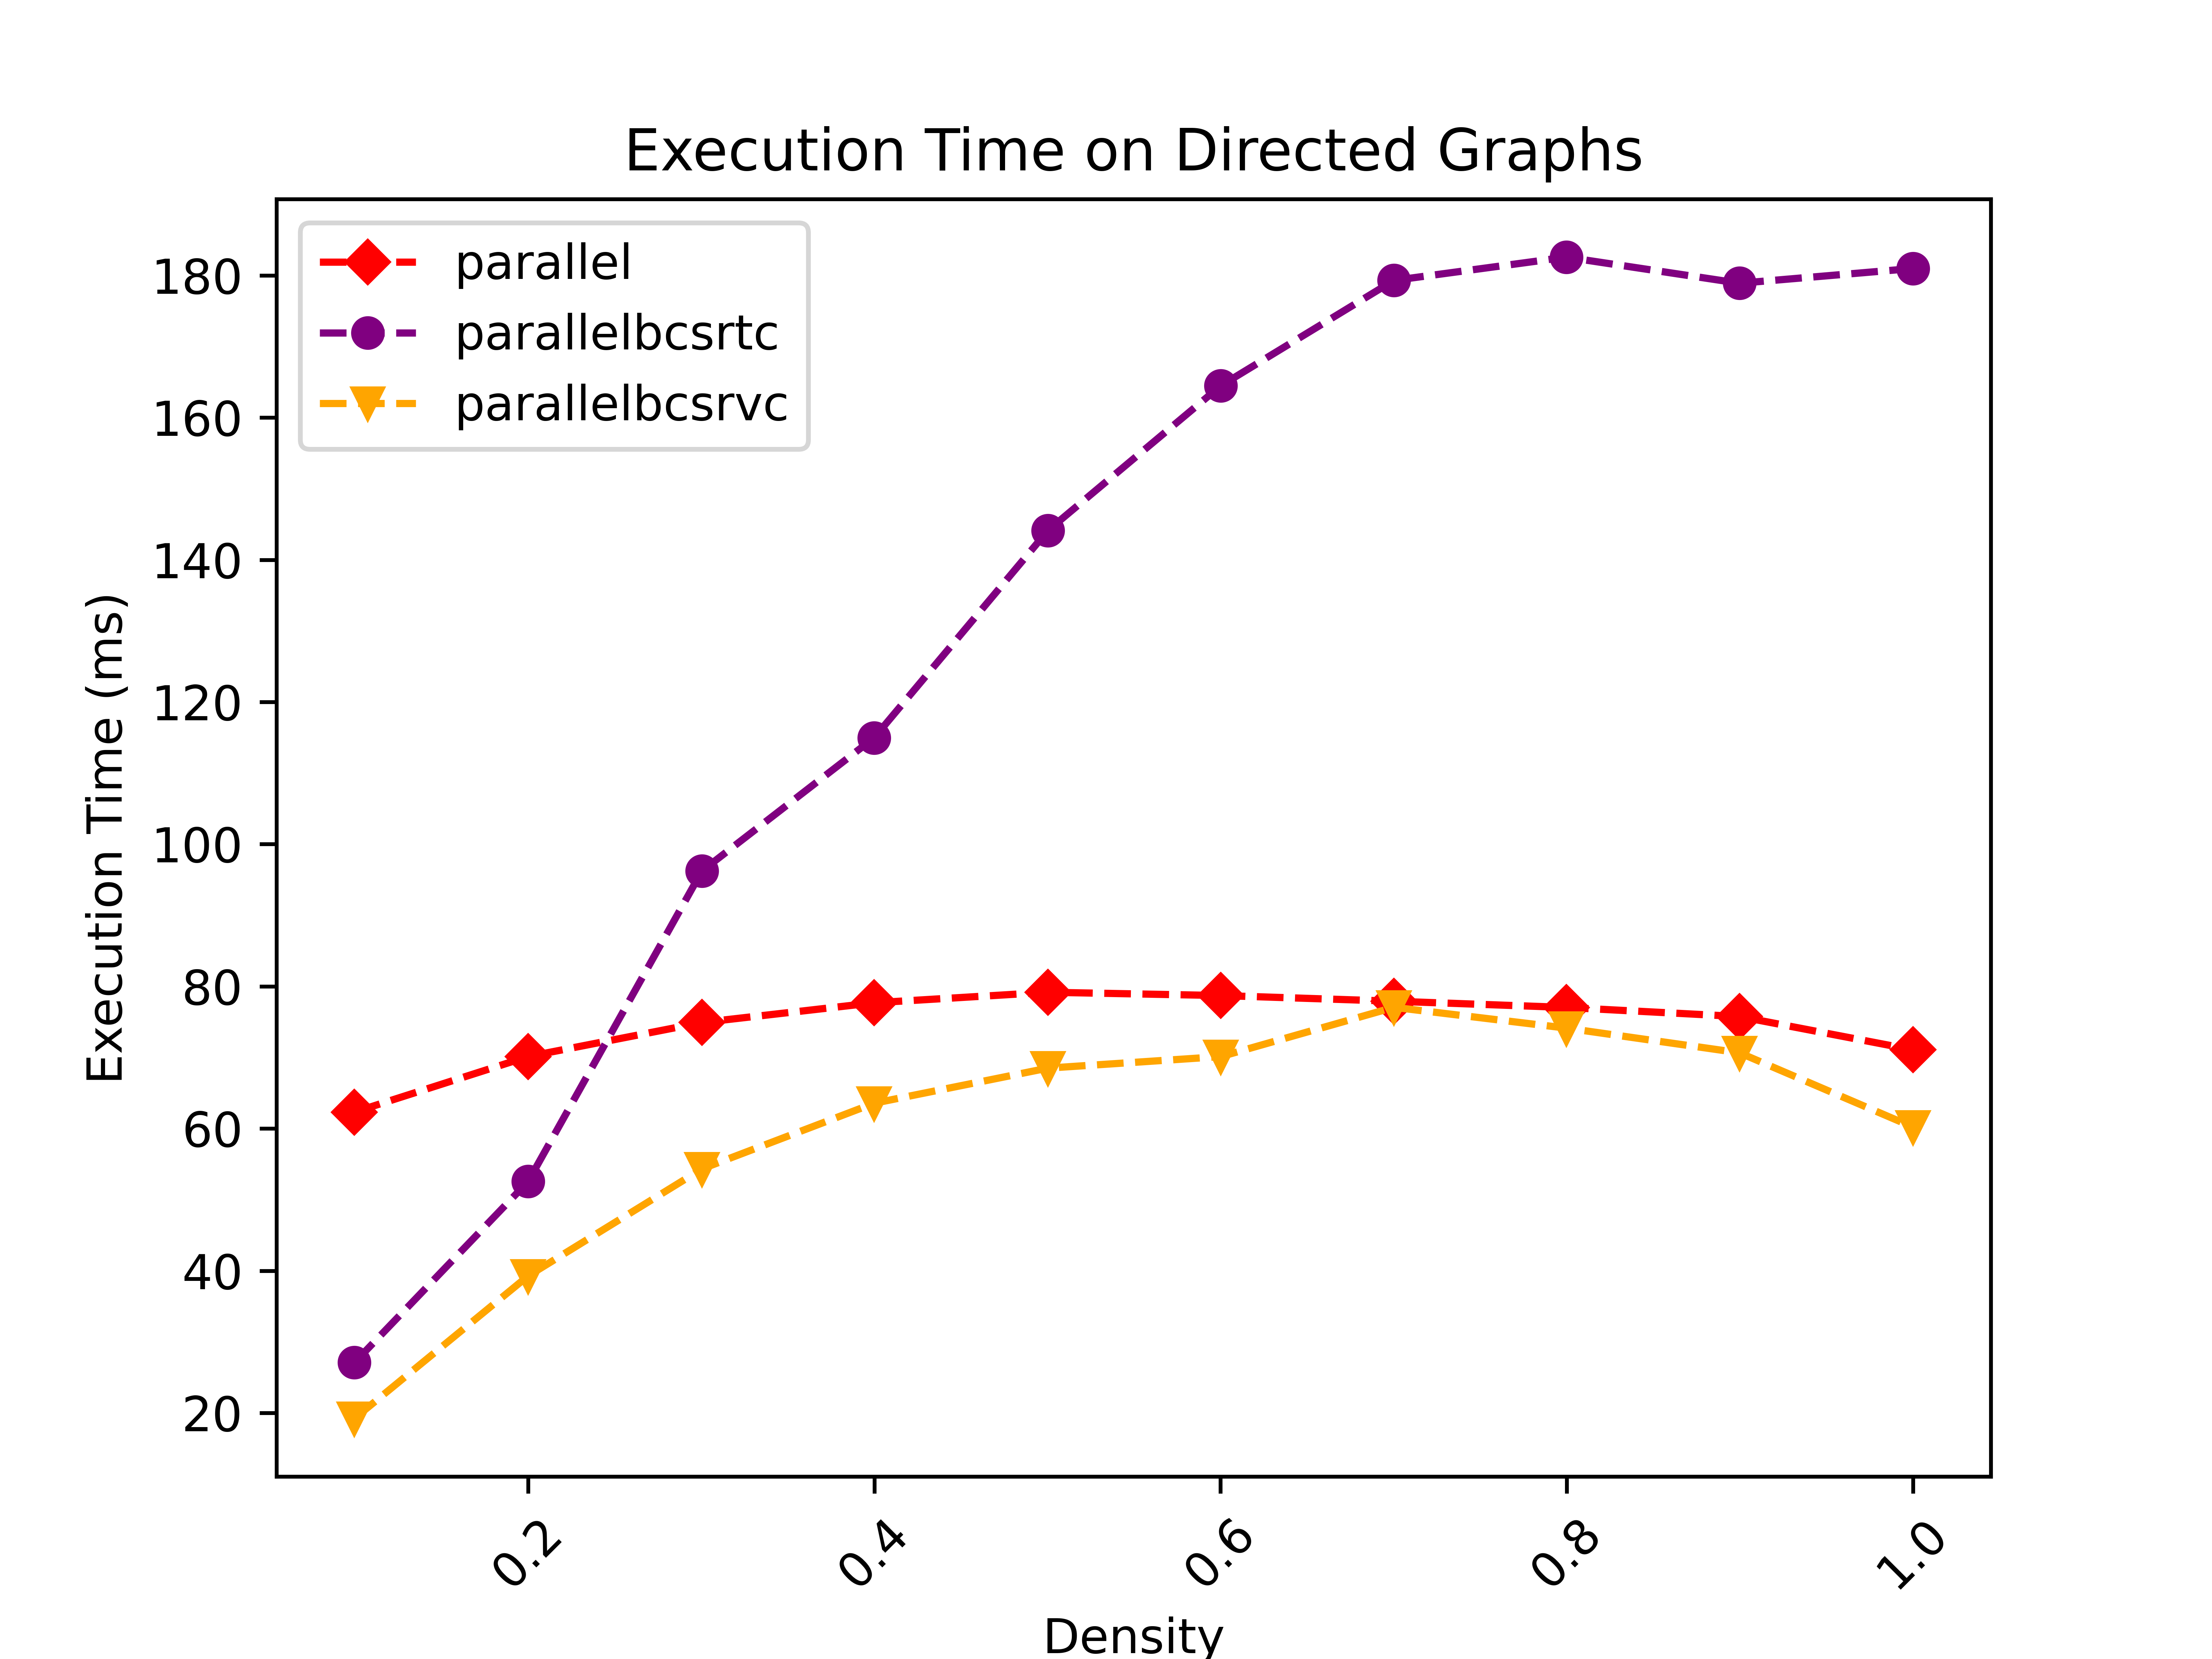
\includegraphics[width=0.7\linewidth]{images/execution_time_density.png}
        \caption{Tempo di esecuzione dei vari algoritmi con grafi diretti a densità variabile}
        \label{fig:exec-time-density}
    \end{figure}





\newpage
Discussione dei risultati
Risultati per test a grafo crescente in numero di nodi
I test eseguiti su grafi con numero di nodi crescente hanno prodotto risultati interessanti, sia per quanto riguarda le versioni parallele dell'algoritmo Push-Relabel applicato a grafi diretti che indiretti.

Grafici di confronto
I grafici di confronto tra le diverse versioni dell'algoritmo mostrano che, all'aumentare del numero di nodi, le prestazioni differiscono notevolmente tra grafi diretti e indiretti.

Grafi diretti: Si osserva che le versioni parallele dell'algoritmo Push-Relabel ottimizzate per grafi diretti tendono a scalare meglio rispetto ai grafi indiretti. Questo comportamento è attribuibile alla struttura delle connessioni nei grafi diretti, che facilita una migliore suddivisione del lavoro tra i thread. Nei grafici, si nota un aumento delle prestazioni fino a un certo numero di nodi, dopo il quale si osserva una stabilizzazione o addirittura un degrado delle prestazioni a causa della crescente complessità delle operazioni di comunicazione e sincronizzazione tra i processori.

Grafi indiretti: Nei grafi indiretti, invece, l'efficienza complessiva è minore. Le versioni parallele ottimizzate per grafi indiretti mostrano un comportamento meno lineare, con una crescita più marcata del tempo di esecuzione all'aumentare del numero di nodi. Questo è probabilmente dovuto alla maggiore interdipendenza tra i nodi nei grafi indiretti, che limita il grado di parallelismo sfruttabile.

Commenti
Per entrambi i tipi di grafo, si osserva un significativo miglioramento delle prestazioni delle versioni parallele rispetto a quelle sequenziali, ma questo beneficio tende a ridursi con l'aumento esponenziale del numero di nodi.
Le prestazioni migliori si ottengono con grafi diretti e un numero medio di nodi, dove il parallelismo è massimizzato senza incorrere in eccessiva latenza dovuta alla sincronizzazione.
Nei grafici di confronto, si osserva che per grafi con un numero di nodi particolarmente elevato, il tempo di esecuzione tende a saturare, evidenziando i limiti intrinseci del parallelismo in presenza di una complessità computazionale crescente.
Risultati per test a grafo con densità crescente
L'esecuzione di test su grafi con densità crescente (numero di archi in proporzione al numero di nodi) ha rivelato alcuni pattern distintivi per quanto riguarda le prestazioni dell'algoritmo Push-Relabel parallelo.

Grafico
Nel grafico che confronta i tempi di esecuzione in funzione della densità del grafo, si osservano due andamenti principali. La matrice di adiacenza con un tempo pressoché costante e la struttura BCSR (Blocked Compressed Sparse Row), che mostra un tempo crescente con la densità.

Osservazioni e possibili spiegazioni
Matrice con tempo costante: L'implementazione dell'algoritmo che utilizza una matrice di adiacenza mantiene tempi di esecuzione pressoché costanti con l'aumentare della densità del grafo. Questo comportamento è dovuto al fatto che, in una matrice, l'accesso ai dati è diretto e non dipende dalla densità del grafo, ma solo dalla dimensione della matrice stessa. Dunque, nonostante un aumento del numero di archi, il tempo necessario per l'accesso e la manipolazione degli elementi non varia significativamente.

BCSR con tempo crescente: Nelle implementazioni che utilizzano la struttura BCSR, si osserva invece un aumento del tempo di esecuzione proporzionale alla densità del grafo. Ciò è spiegabile dal fatto che, con l'aumento della densità, la struttura BCSR diventa progressivamente più complessa e richiede più tempo per la gestione degli archi compressi. In questa struttura, ogni blocco richiede operazioni aggiuntive di lettura e scrittura, il che penalizza le prestazioni quando il numero di archi diventa molto elevato.

Densità elevate, stessi tempi: Un punto interessante evidenziato dai risultati è che, per densità molto elevate, i tempi di esecuzione tendono a convergere tra le varie implementazioni. Questo fenomeno può essere interpretato come un limite superiore intrinseco per entrambe le strutture dati: quando un grafo diventa altamente connesso, i benefici di strutture sparse come BCSR vengono annullati e la complessità complessiva del grafo impatta in maniera uniforme tutte le implementazioni.

Linea viola per BCSR senza ottimizzazioni complete: Nel grafico, si nota una linea viola corrispondente alla versione BCSR non completamente ottimizzata. Questa variante si rivela particolarmente inefficiente e, in definitiva, inutile per grafi con densità elevata, in quanto non riesce a sfruttare adeguatamente le proprietà di compressione della struttura BCSR. Questo risultato conferma che l'ottimizzazione completa delle strutture dati è essenziale per ottenere prestazioni competitive, soprattutto con grafi densi.

Considerazioni finali
I test sui grafi a densità crescente e quelli a numero di nodi crescente forniscono indicazioni complementari sull'efficacia dell'algoritmo Push-Relabel parallelo. Nei grafi a numero di nodi crescente, il parallelismo mostra risultati promettenti ma non senza limitazioni dovute alla complessità della comunicazione tra processi. Nei grafi con densità crescente, invece, l'ottimizzazione delle strutture dati gioca un ruolo determinante nelle prestazioni, specialmente con grafi densi dove strutture come BCSR devono essere attentamente progettate per evitare inefficienze.

In conclusione, le prestazioni dell'algoritmo Push-Relabel parallelo sono fortemente influenzate sia dalla tipologia di grafo che dalle strutture dati utilizzate. La corretta scelta di queste ultime e una buona gestione del parallelismo sono fattori chiave per garantire un'efficace scalabilità dell'algoritmo.